\begin{post}
	\postdata{We didn't start the fire...}{2011}{10}{11}{22}{50}{17}
	\begin{content}
\begin{blockquote}Lots of work\\
Take a break\\
Fireworks\\
Boom bang bang!
\end{blockquote}

\textit{I couldn't resist to put this little pop-culture reference here, even though I doubt that someone will recognize it:)}

On Saturday we went to see the annual Seoul International Fireworks Festival, that took place in the Yeouido Hangang Park, at the bank of the Han river. It is a one day event, organized by a explosives company called Hanwha, and this year there were teams from Korea, Japan and Portugal showing their fireworks skills.

Our Korean friends told us that it is going to be crowded. And they were right. When we saw the masses of people in the subway we realized that leaving the dorm at 6pm was maybe a little too late, considering that the first show was scheduled for 7:30pm. After getting to the subway line 5, we quickly found out that "crowded" was a mere underestimation of the situation. Everybody in Seoul went to see the fireworks. Or at least it seemed so.

\begin{figure}[h]
\centering
\subfigure[The whole population of Seoul gathered at one subway station]{\fbox{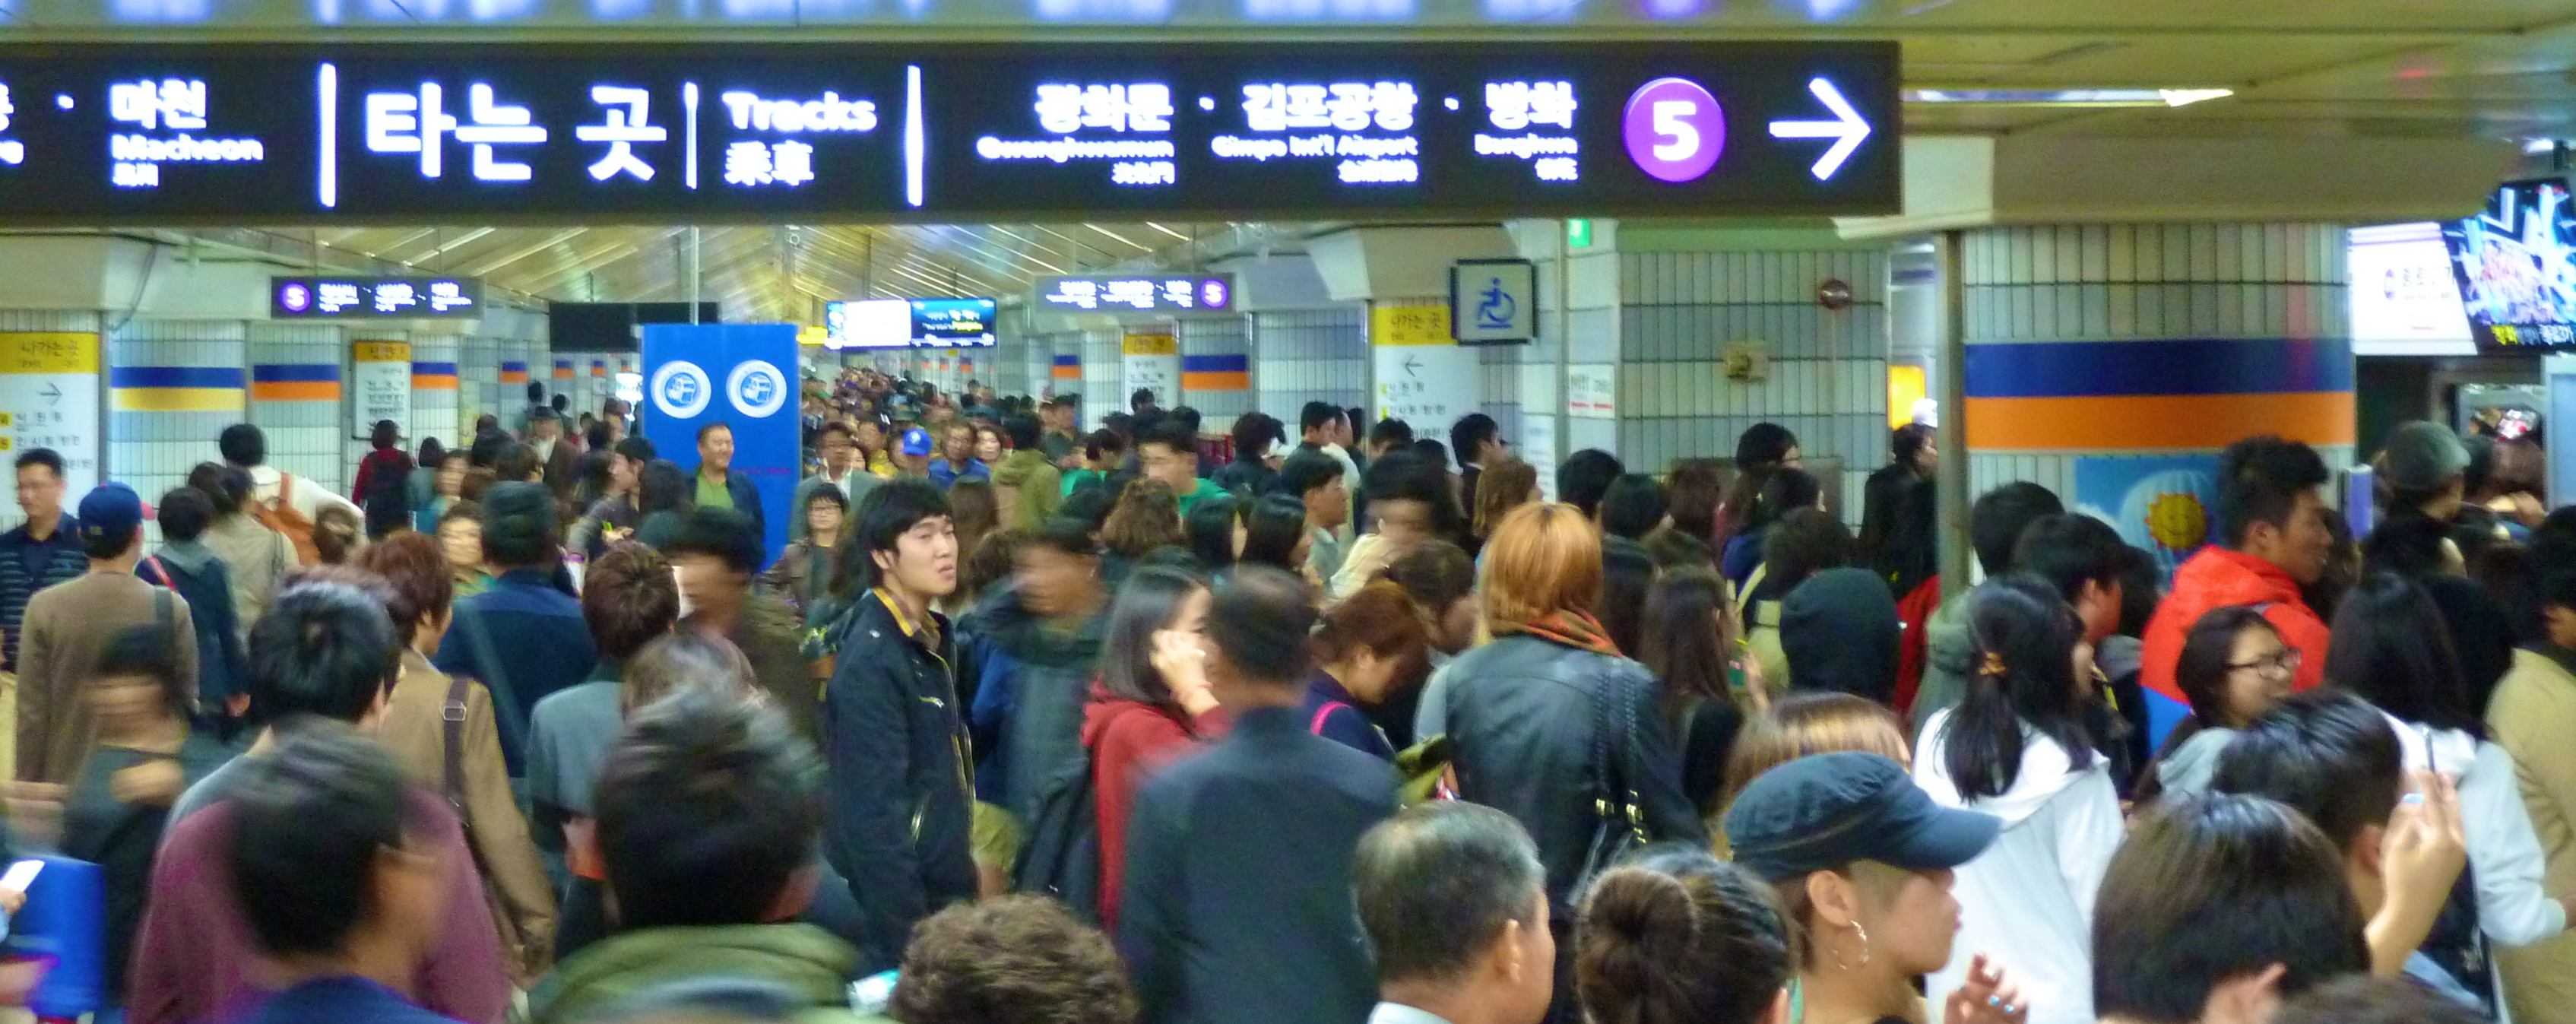
\includegraphics[height=0.245\textwidth]{photos/10/11/p1000693.jpg}}}
\subfigure[Crowding out the escalator]{\fbox{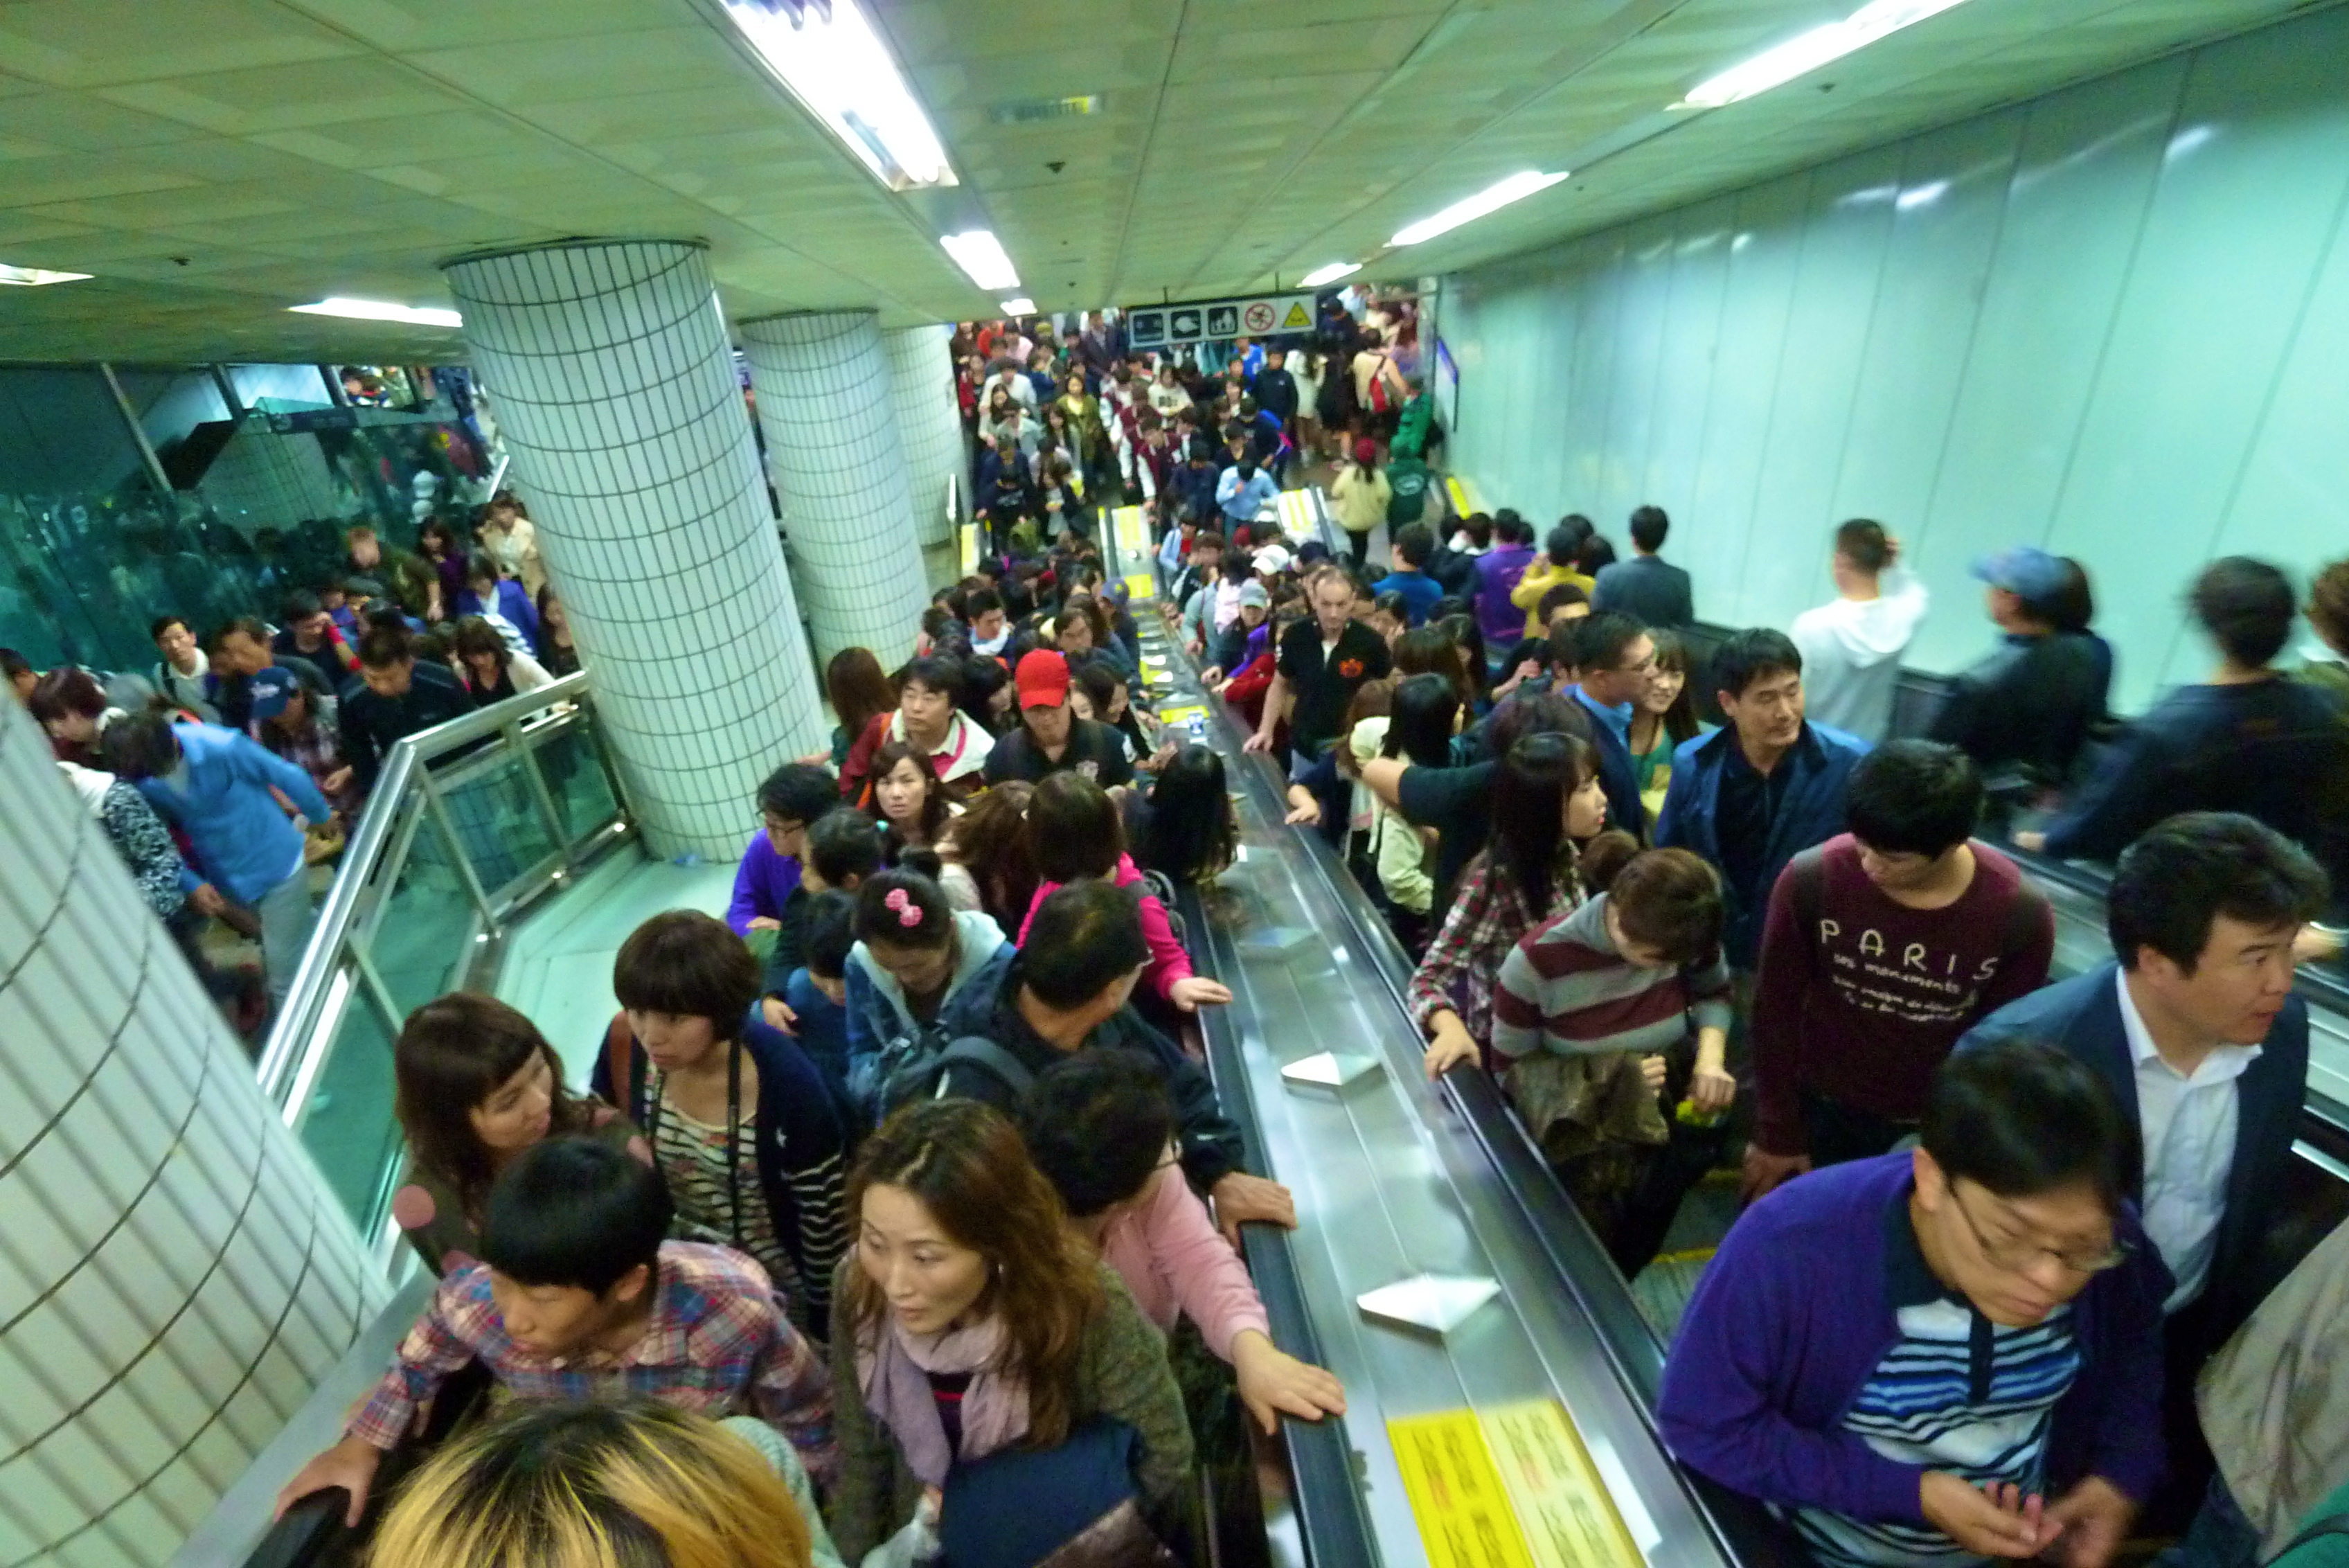
\includegraphics[height=0.245\textwidth]{photos/10/11/p1000703.jpg}}}
\end{figure}

%[caption id="attachment_217" align="aligncenter" width="550" caption="The whole population of Seoul gathered at one subway station"]<a href="http://soulexchange.wordpress.com/2011/10/11/we-didnt-start-the-fire/p1000693/" rel="attachment wp-att-217"><img class="size-medium wp-image-217" title="The whole population of Seoul gathered at one subway station" src="http://soulexchange.files.wordpress.com/2011/10/p1000693.jpg?w=550" alt="" width="550" height="218" /></a>[/caption]

Inside of the trains it was like a frotteur's dream. As more and more people were pouring in at each station, it was getting more and more uncomfortable, with people pushing from all sides, trying to get through. This crowd had one advantage, though. Since we were not sure where to get off the train, we simply waited until the sea of people washed us out. At the station the situation repeated — people, people, people. Fortunately, Koreans have anticipated this situation, so the vestibule was full of people in reflective vests with shining \sout{cheering} sticks, that were managing the crowd, trying to distribute the mass of human bodies equally between the subway exits. And honestly, they managed quite well. We were still moving forward, without unnecessary waiting.

%[caption id="attachment_220" align="aligncenter" width="449" caption="Crowding out the elevator"]<a href="http://soulexchange.wordpress.com/2011/10/11/we-didnt-start-the-fire/p1000703/" rel="attachment wp-att-220"><img class="size-medium wp-image-220" title="Crowding out the elevator" src="http://soulexchange.files.wordpress.com/2011/10/p1000703.jpg?w=449" alt="" width="449" height="300" /></a>[/caption]

The situation outside was fortunately better — some streets were closed for traffic, so there was enough space for all the people to spread out. Soon after we left the subway, the first show started, so we just found some place where we could see the sky and watched the fireworks. I don't know if it was the Japanese one or the Portuguese, though. After the first one we moved to the bridge, close to which was the pier the fireworks was launched from. The police was trying to keep the traffic going, however, since only one line was open and there were people running across the bridge all the time, it was quite difficult. Later on we managed to get across the bridge, which really gave us nice view on the fireworks. I tried to take some pictures, however, it would require a tripod and a SLR to make it look awesome. So it is just nice...

\begin{figure}[h]
\centering
\subfigure{\fbox{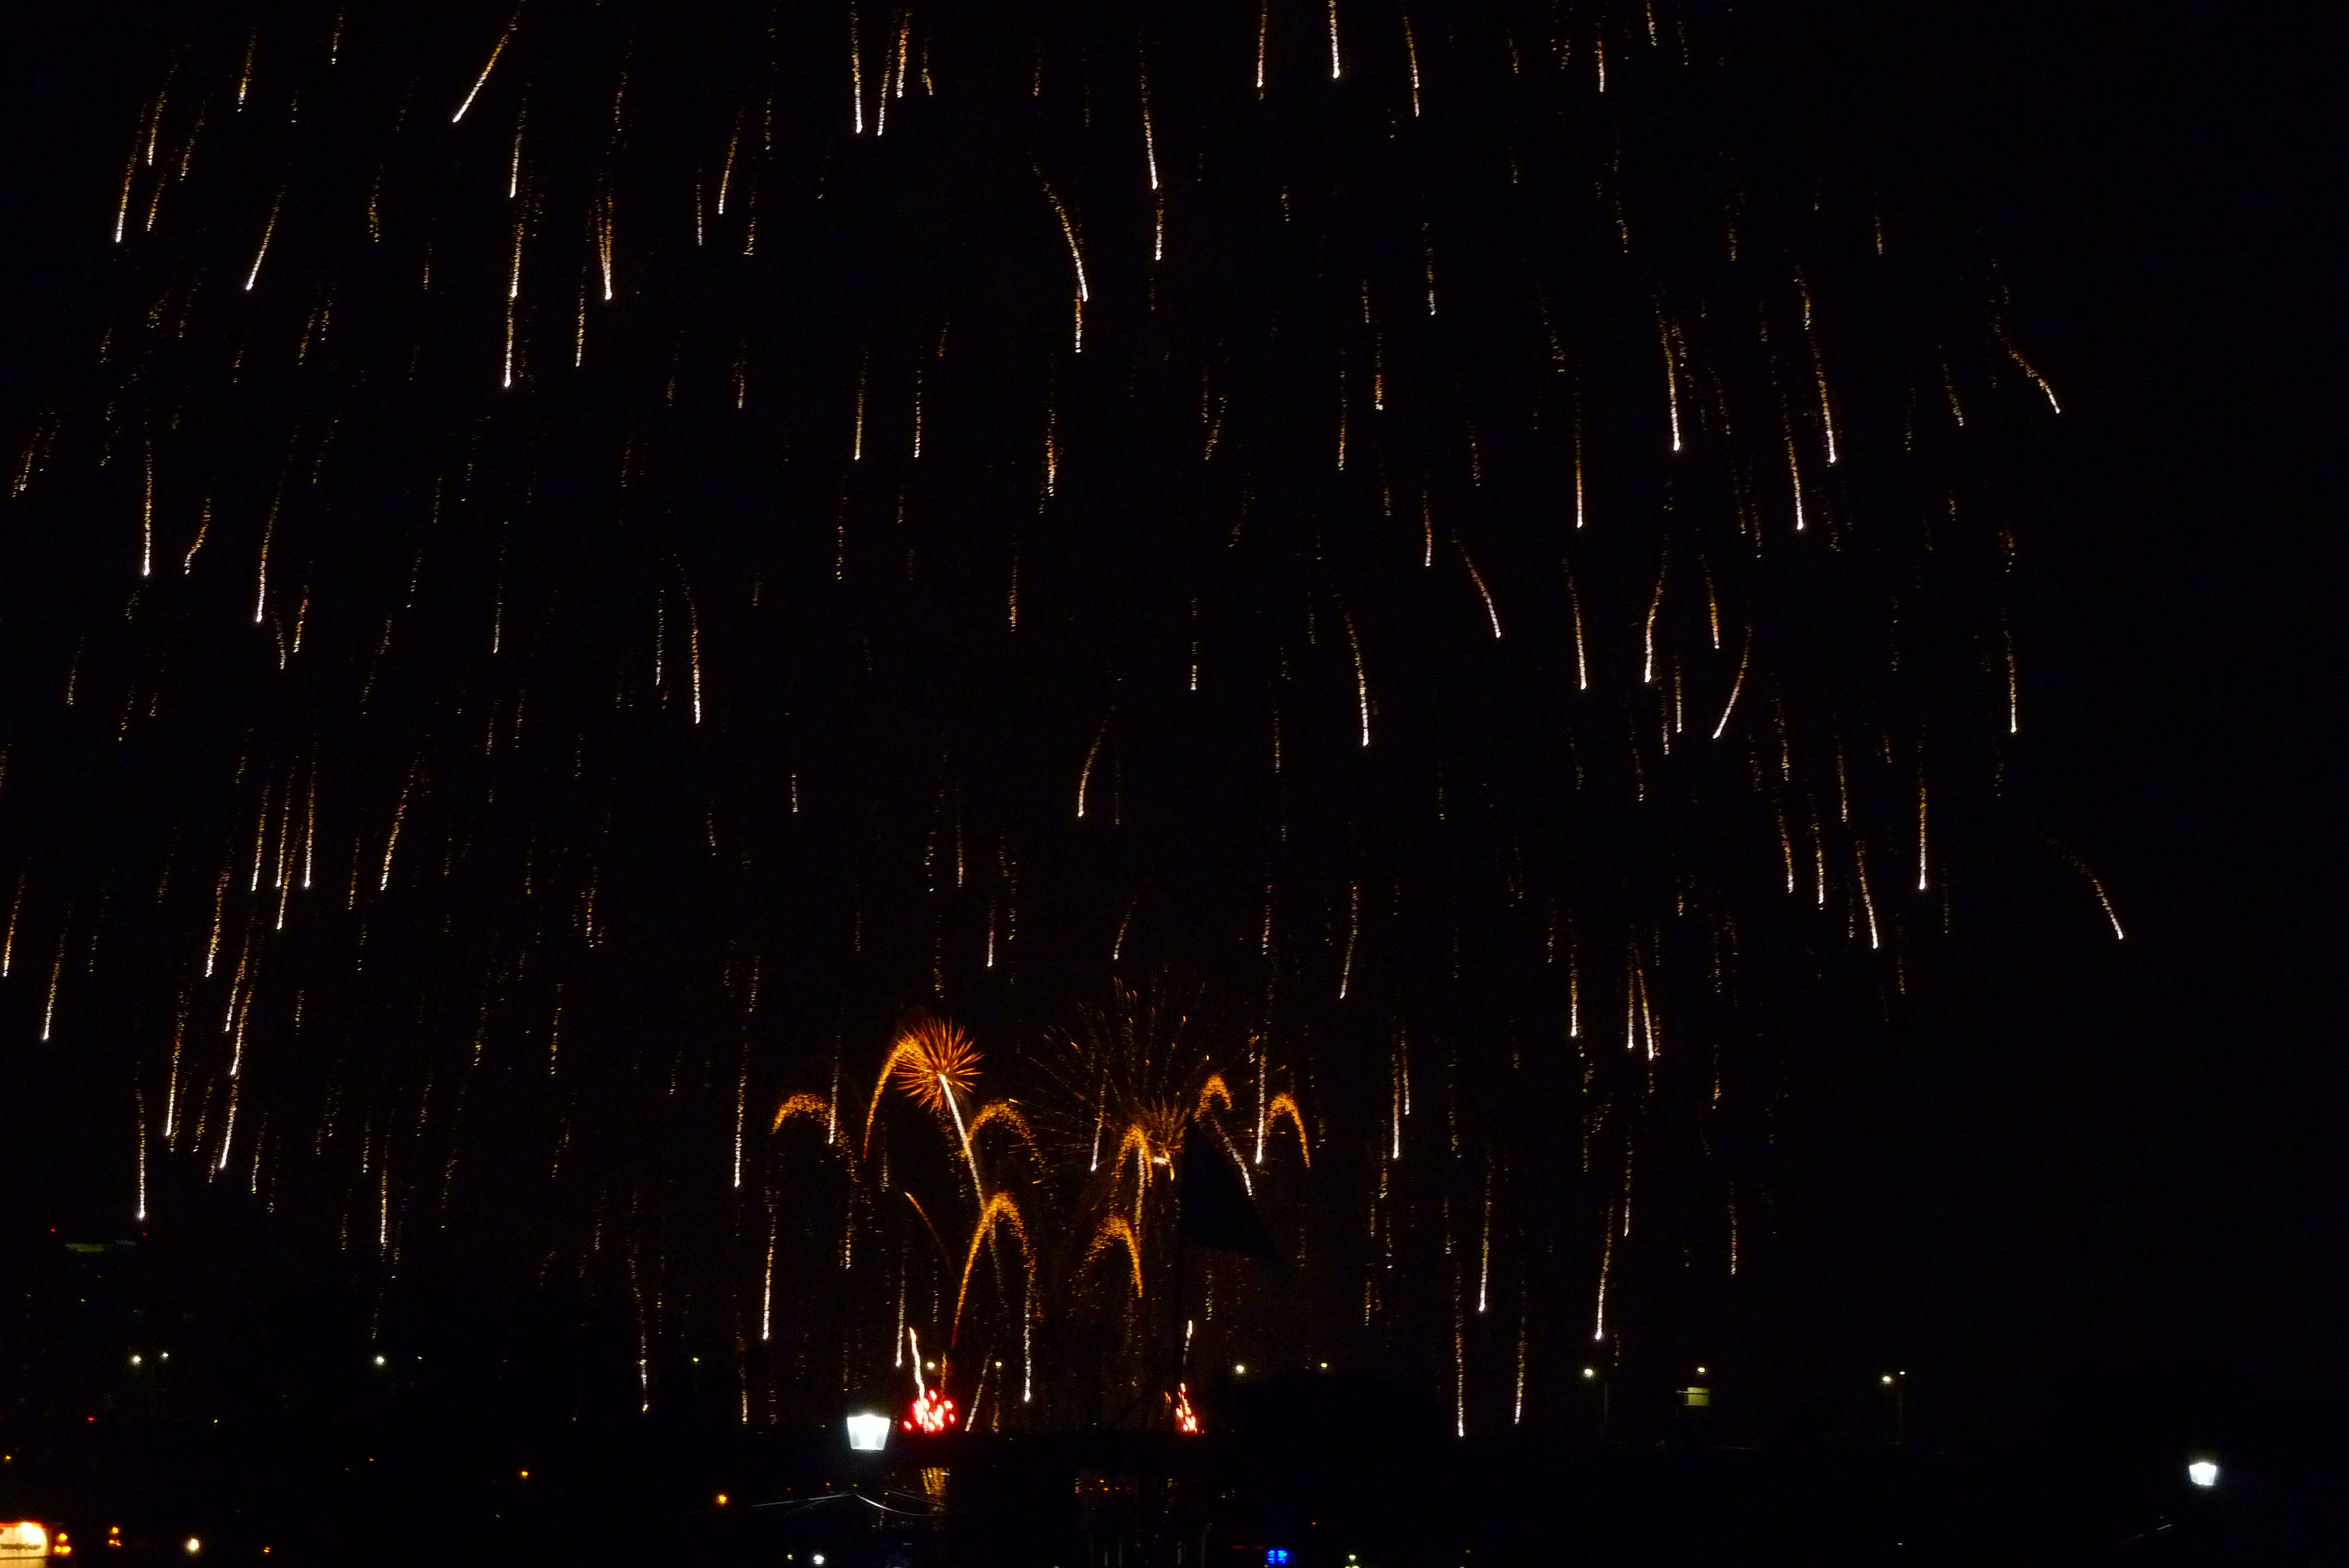
\includegraphics[height=0.36\textwidth]{photos/10/11/P1000757.jpg}}}
\subfigure{\fbox{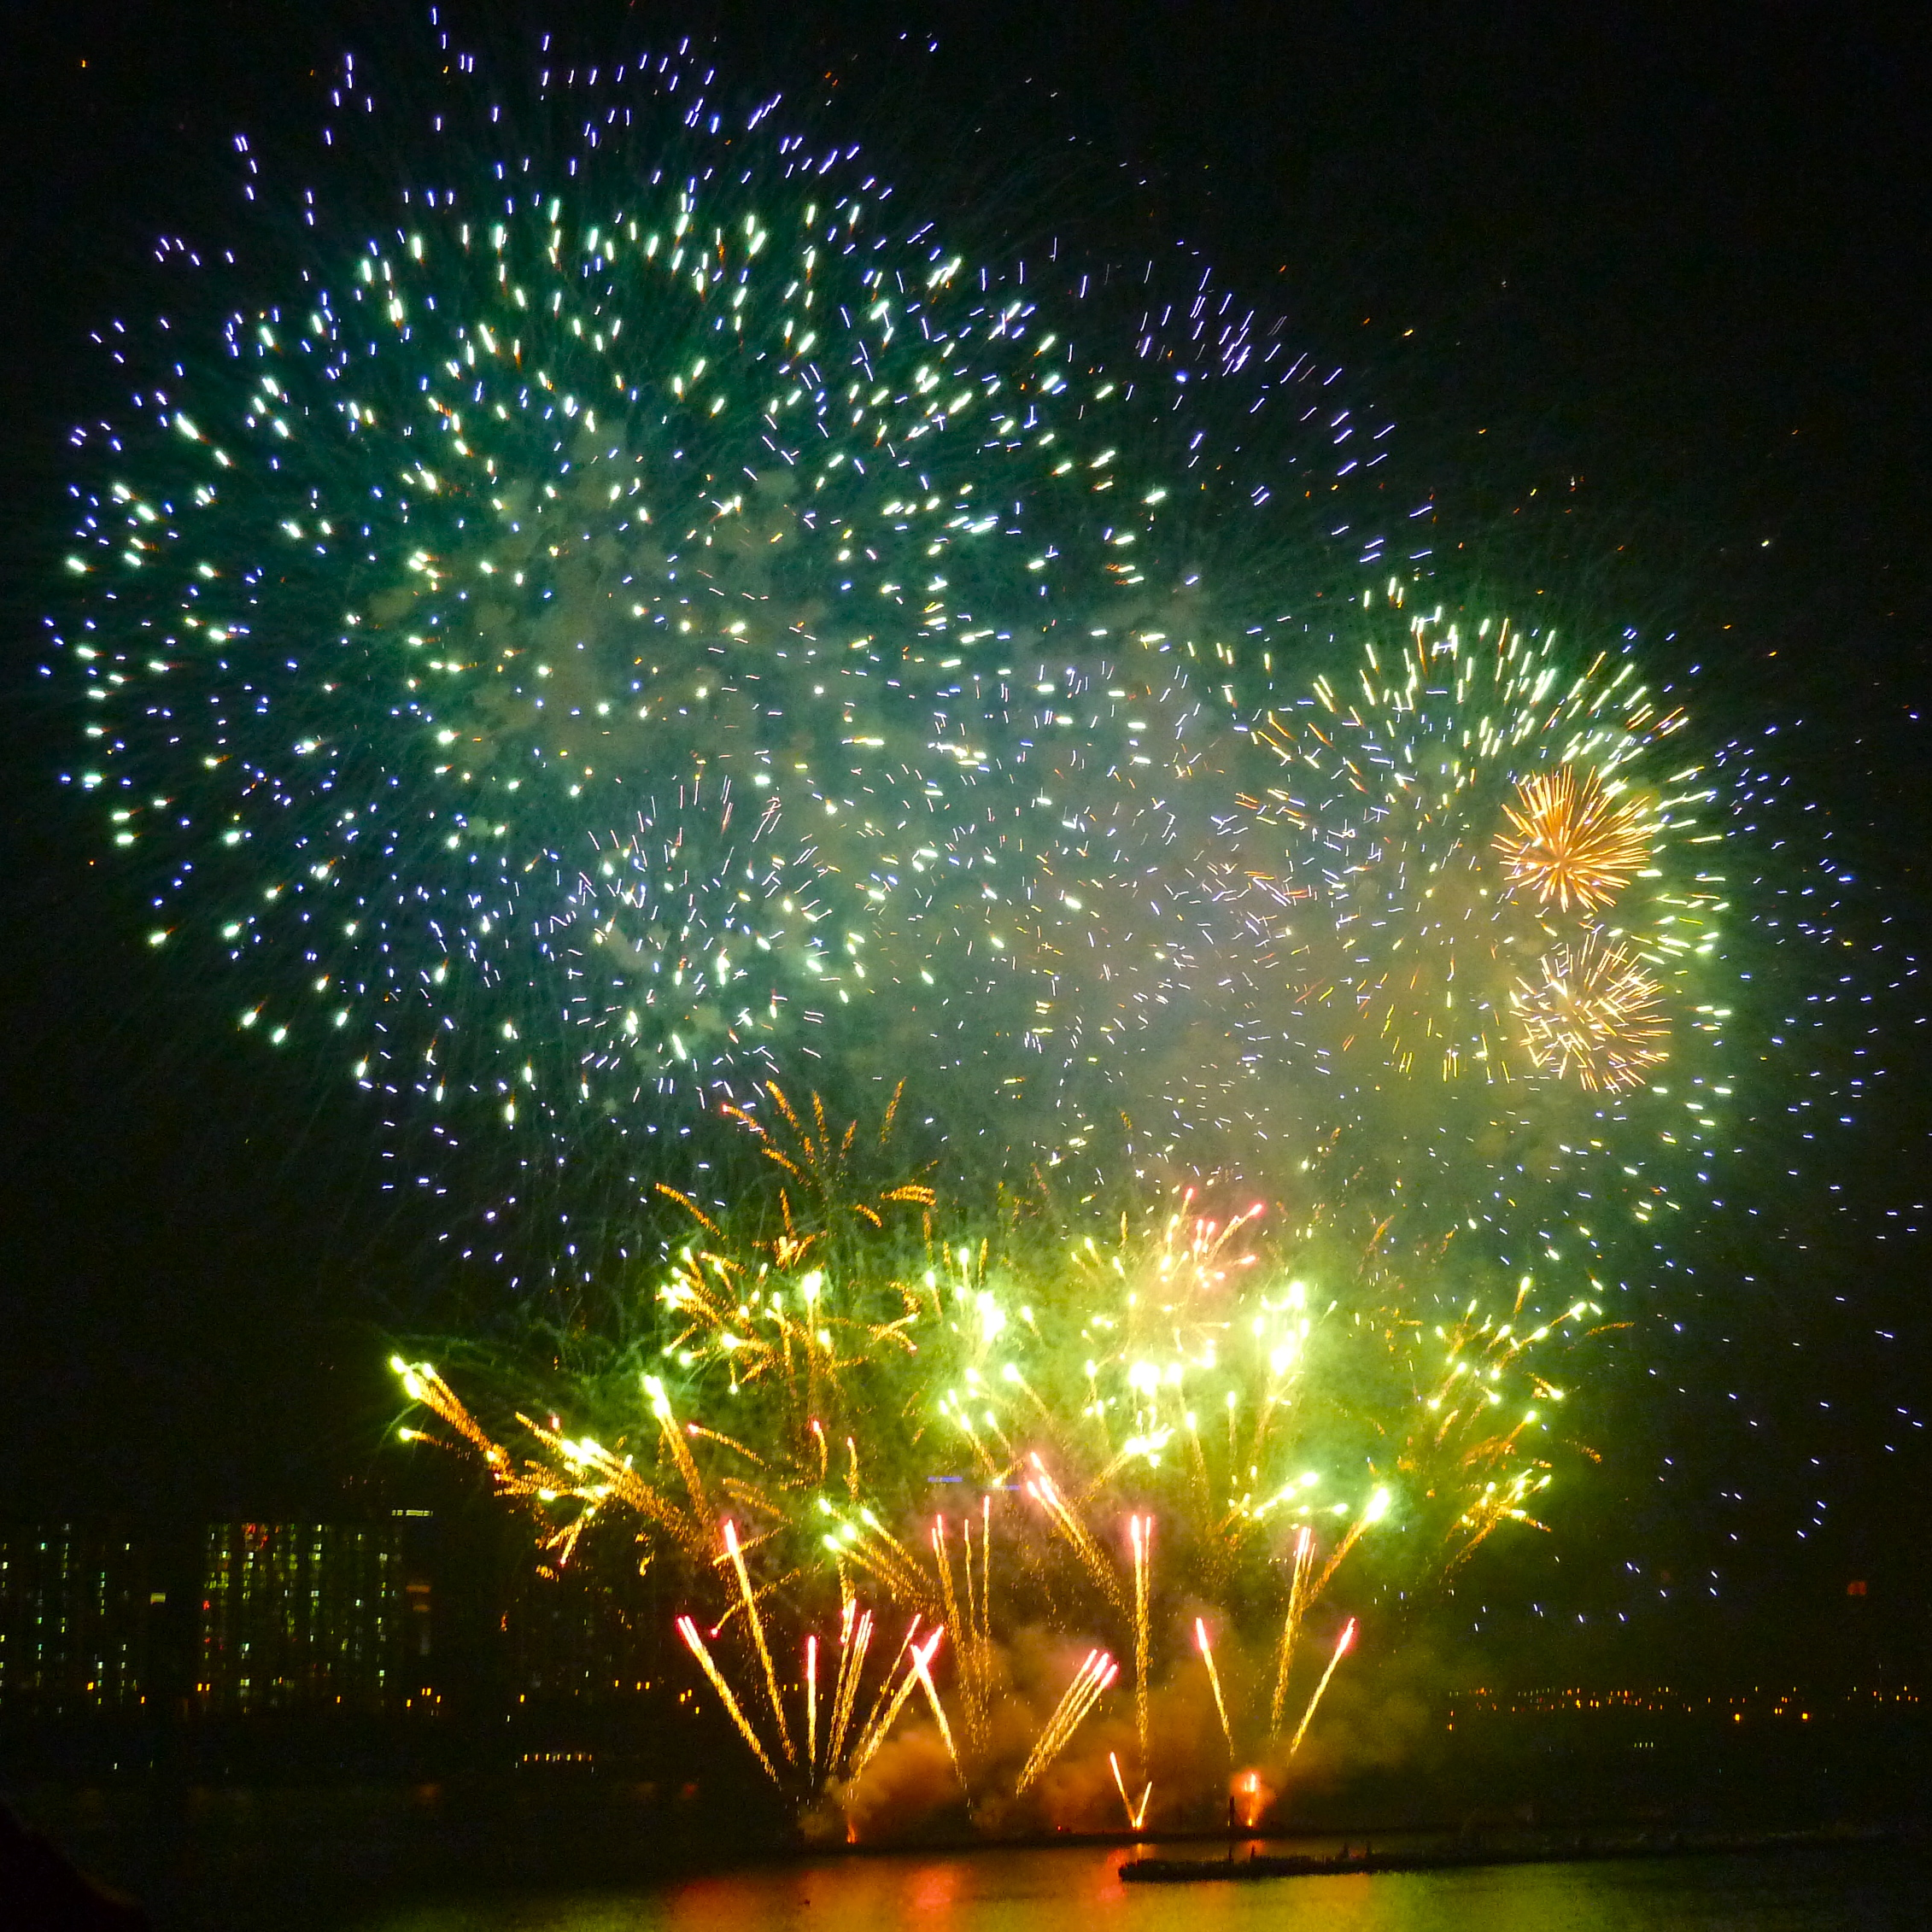
\includegraphics[height=0.36\textwidth]{photos/10/11/P1000809.jpg}}}
\caption{The fireworks}
\end{figure}

After the fireworks we went to the building "63", which used to be the tallest building in Korea, or even Asia, where we had a dinner and then we set off for \sout{home} the dorm. The problem was that there was still a lot of people, so when we came to the subway station, the entrance was simply closed and guarded by police and subway officials. To prevent overcrowding of the subway, they let people in only when there was enough space. They also distributed people between the different entrances, so none would get clogged. Well, it worked quite well. I have to admit, Koreans are so orderly and well organized!</span></p>

\begin{figure}[h]
\centering
\subfigure[4xD + 1xCZ]{\fbox{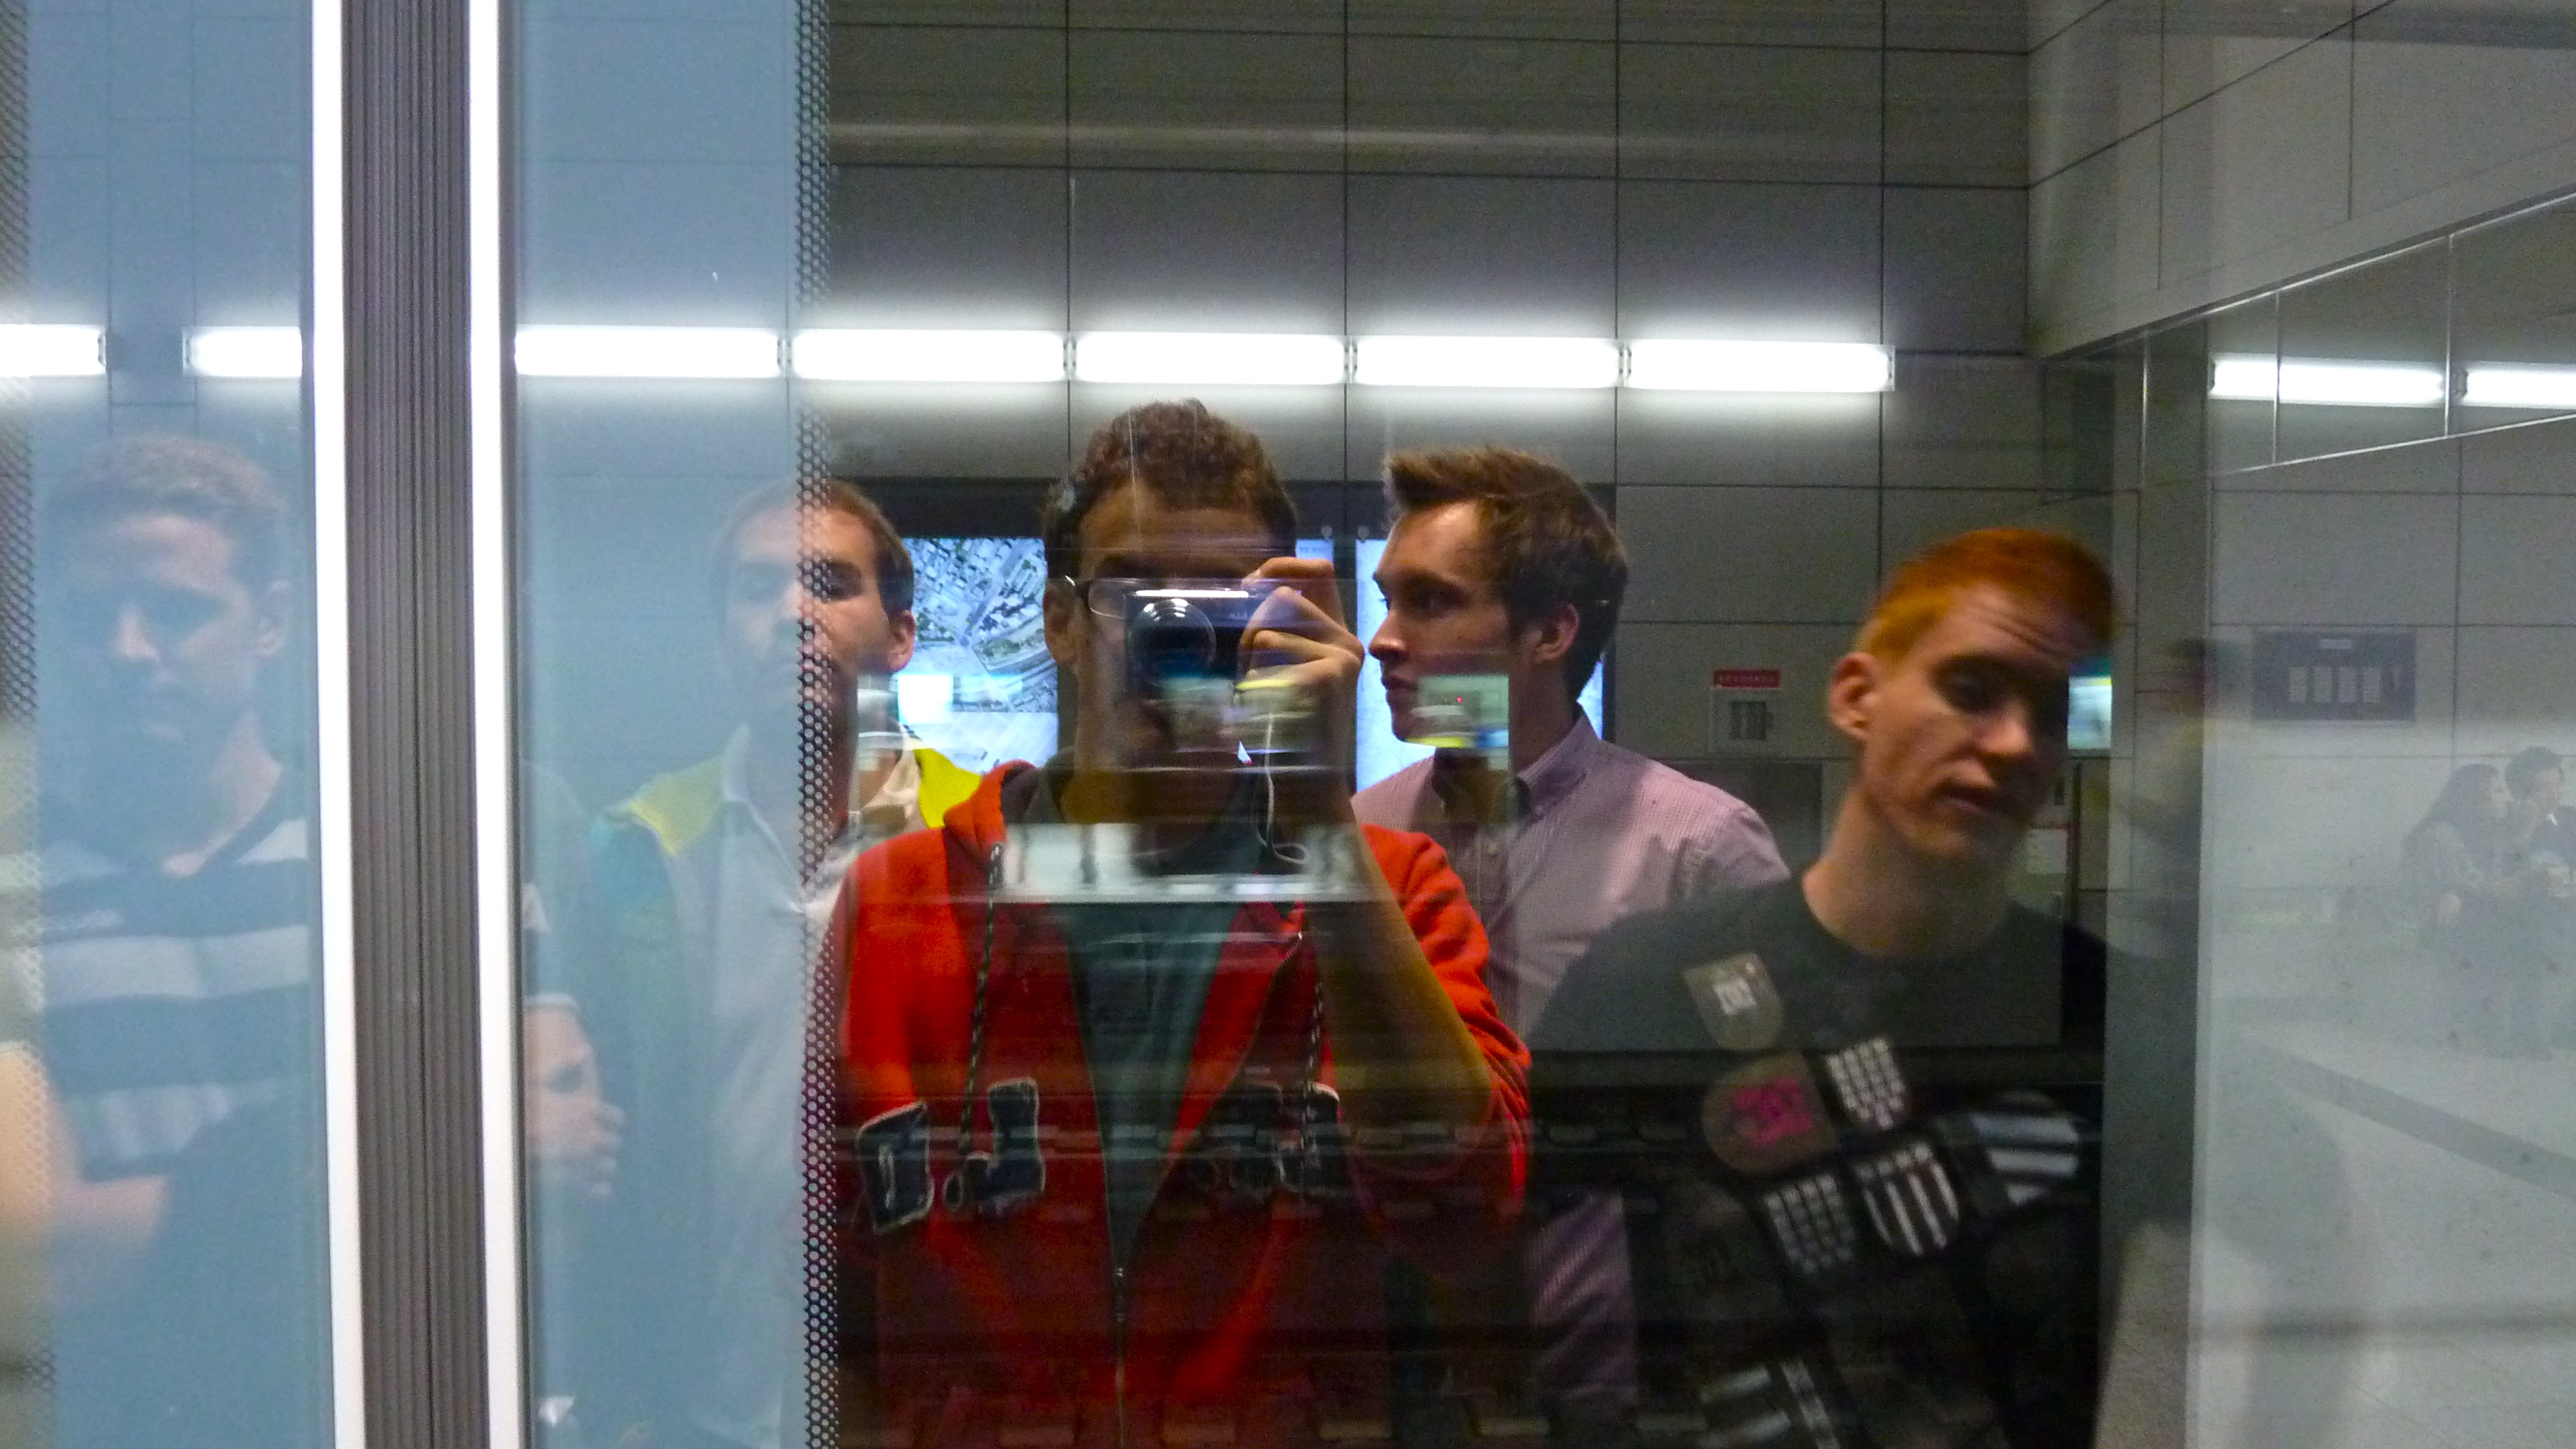
\includegraphics[width=0.485\textwidth]{photos/10/11/P1000910.jpg}}}
\subfigure[Crowded Noriangjin station]{\fbox{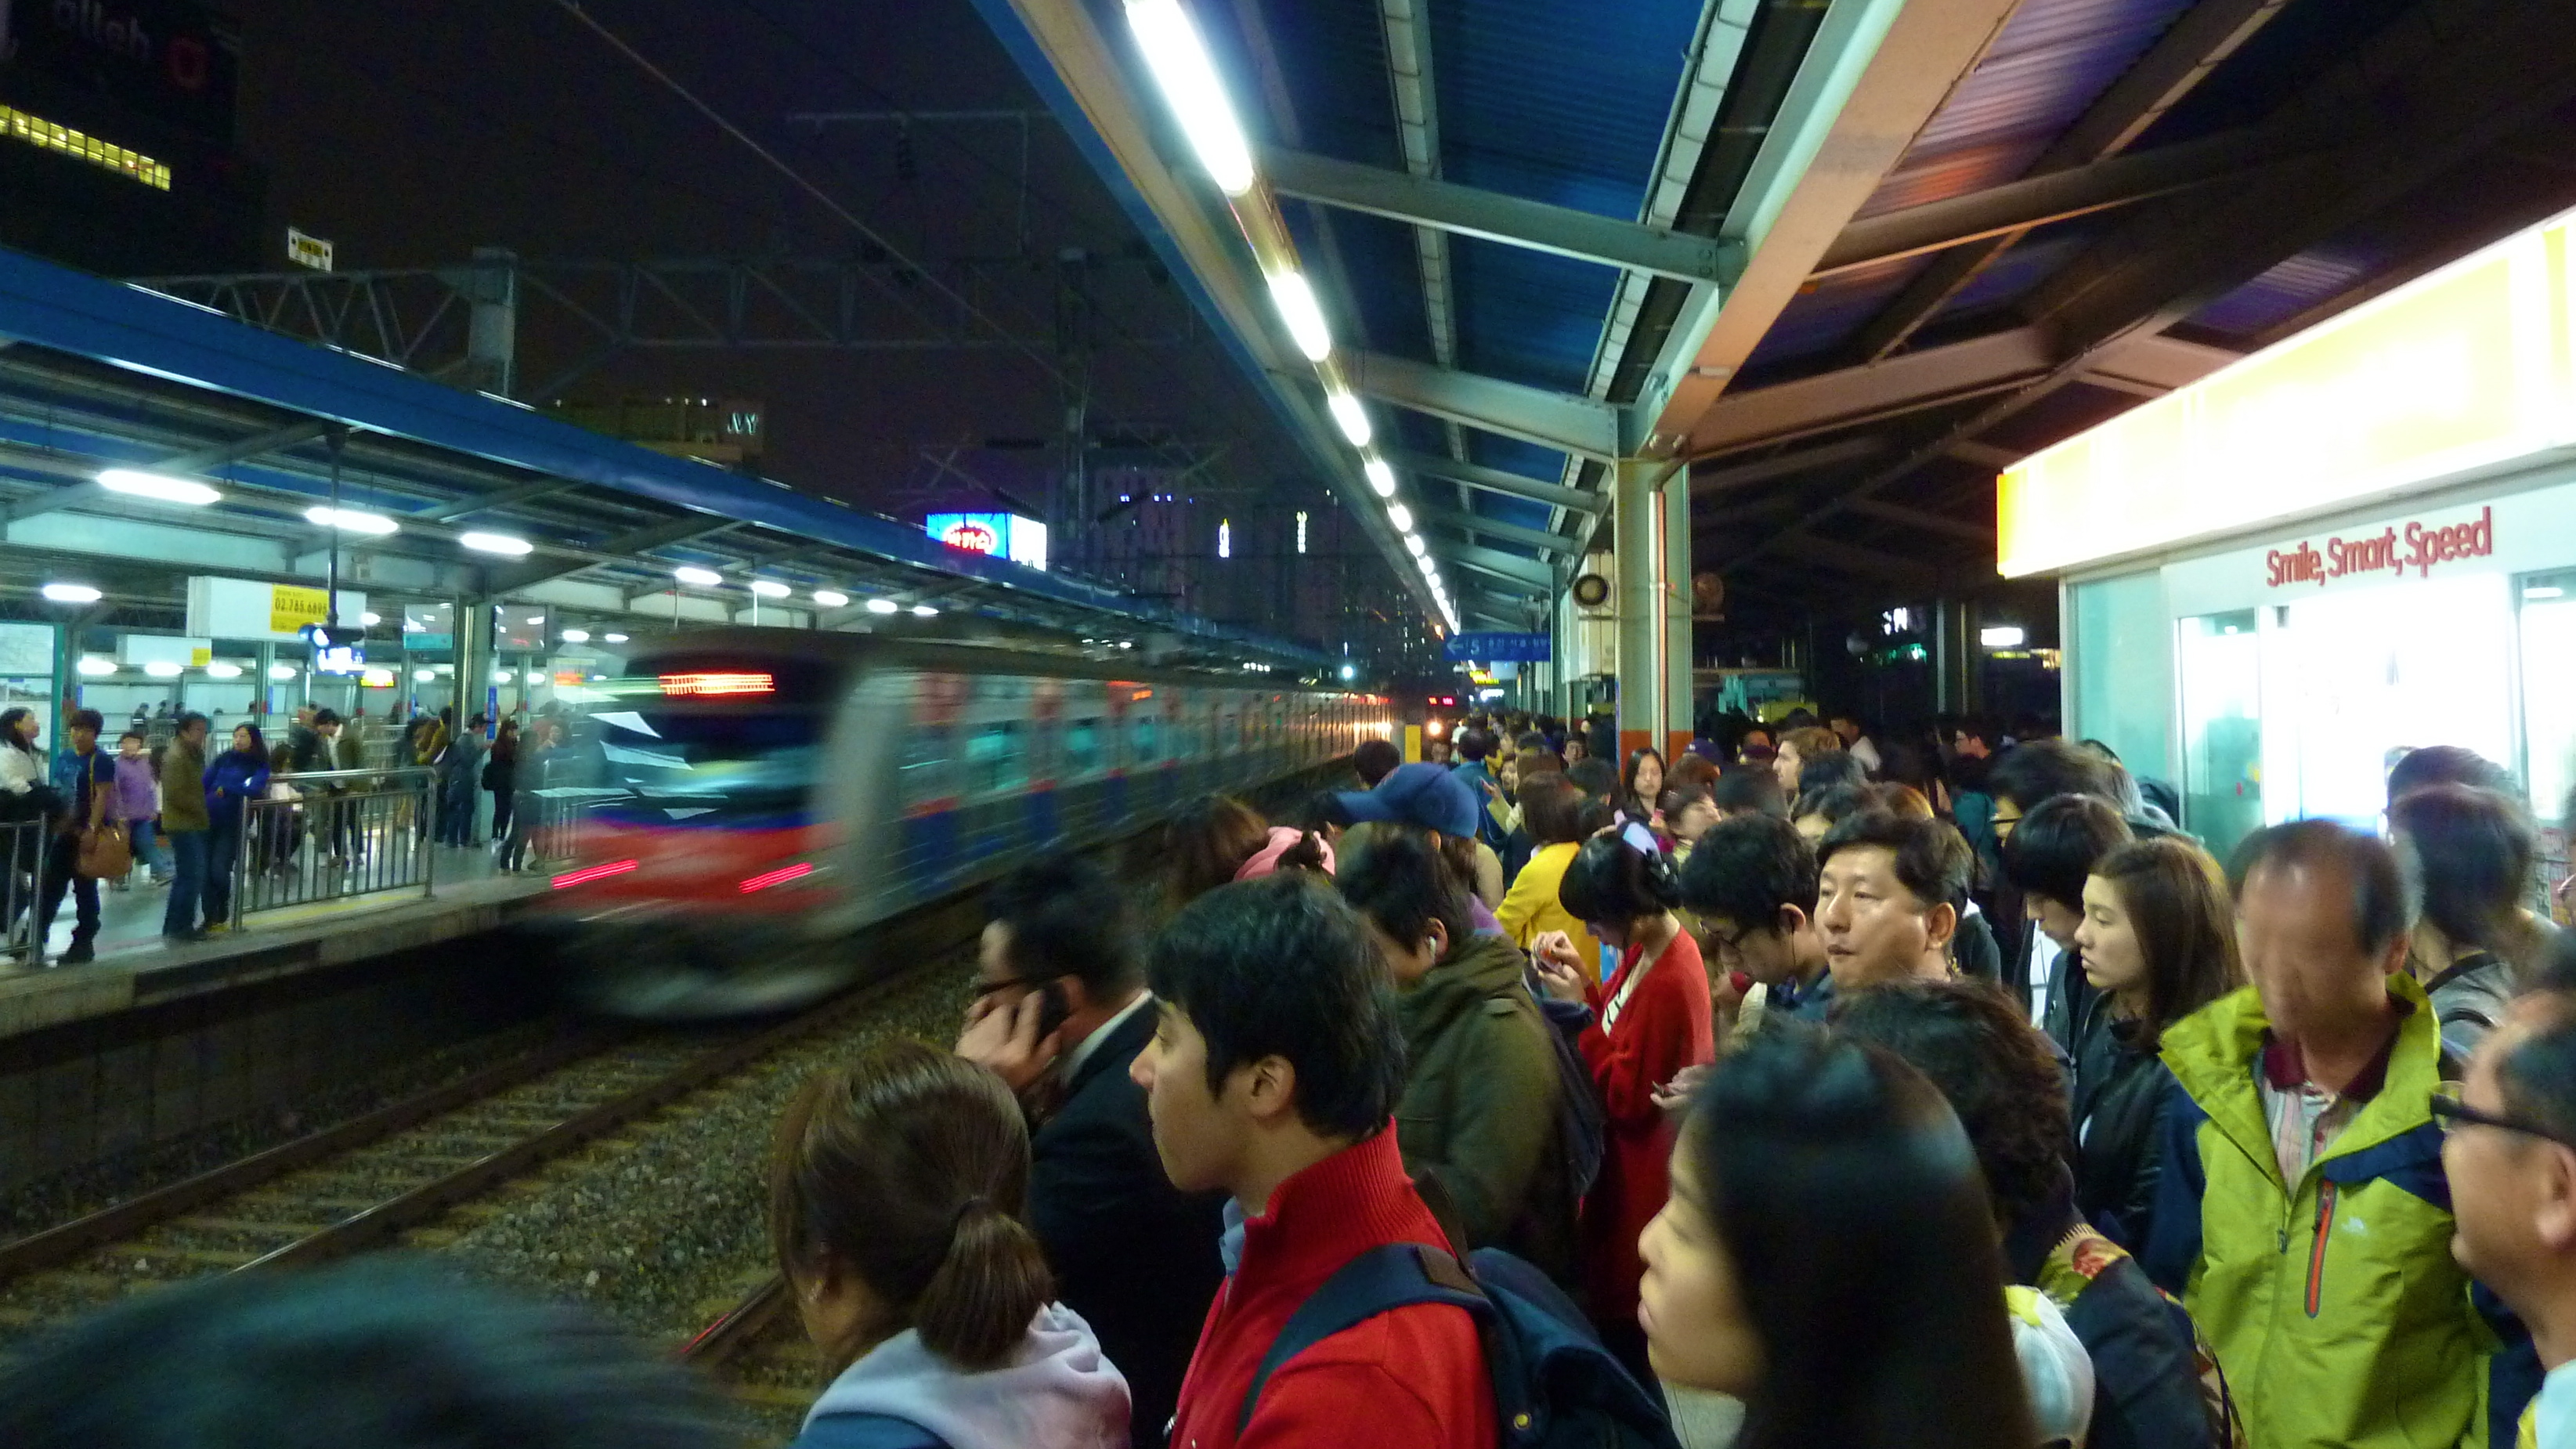
\includegraphics[width=0.485\textwidth]{photos/10/11/P1000918.jpg}}}
\end{figure}

The ride back was one of the moments when you just wish you were home, because you are tired and the subway is packed and everything is annoying etc. But we made it, and the final walk from Hoegi, with a short stop for a "meat on the stick" was a nice ending to a tiring afternoon.



	\end{content}
\end{post}
